%! Author = Saeid Yazdani
%! Date = 07/20/2023


\section{Output Driver Stage}
\label{sec:output-driver-stage}

In any power supply, the output driver stage is the most critical
building blocks as it is directly responsible for delivering
the power and any shortcomings in this section of the system can
render the whole system ineffective, even if the other building blocks of
the system are perfectly designed and developed.
Hence, this section will cover more details in comparison to other sections of
this chapter.

\autoref{fig:driver-stage-diagram} shows the high-level diagram of the
proposed three-stage amplifier chain:

\begin{enumerate}[topsep=8pt,itemsep=4pt,partopsep=4pt, parsep=4pt]
    \item \textbf{Pre-Amplifier (low-voltage):}
    A low-offset, low-drift, high-precision amplifier provides the initial gain
    to bring the \emph{SET} (desired value) and \emph{ERROR} (actual value)
    signals up to a level that is appropriate for the subsequent stages.

    \item \textbf{Power Amplifier (high-voltage):} Low-drop driver for
    high-voltage levels and providing stable gain at those levels.

    \item \textbf{Source Follower (current-booster):} increases current output
    specially for low-impedance loads and respond effectively to dynamic
    load conditions.

\end{enumerate}

\begin{figure}[t!]
    \centering
    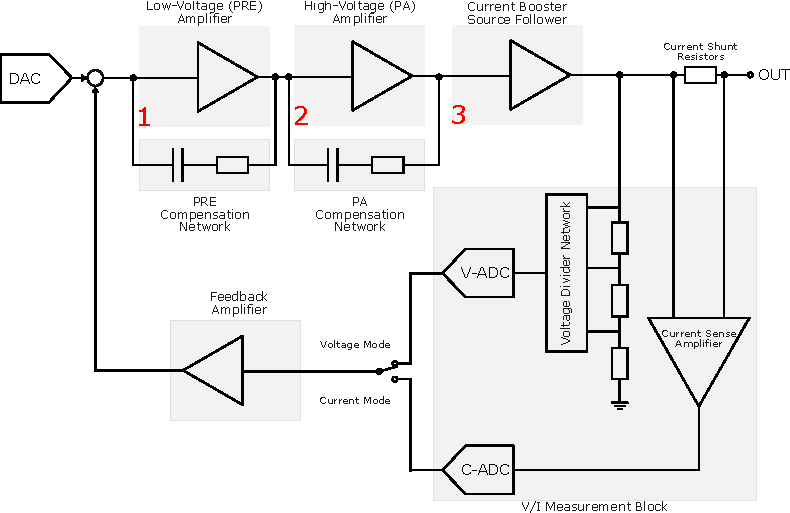
\includegraphics[width=1.0\textwidth]
    {figures/prototype/driver-stage-overview}
    \caption[Three-Stage Driver]{
        Overview of the proposed three-stage driver for system output.
        Low-voltage and high-voltage stages each have their own dynamic
        compensation network as discussed in
        \autoref{subsec:compensation-control-fpga}.
        The output of the driving stages is fed to a voltage and current
        measurement arrangement to calculate deviation from desired setpoint
        and fed this error back into the system for correction.

    }
    \label{fig:driver-stage-diagram}
\end{figure}

\subsection{Design Challenges for the Driver Stage}
\label{subsec:design-challenges-driver-stage}

Major requirements in designing a DPS are stability, controlled slew rate,
wide-band frequency response, cost and availability.
In addition, ATE power supplies must minimize internal heating, as there is
limited space for large heatsinks and sufficient airflow cannot be guaranteed.
Therefore, using a low-drop driver is a priority.

At the time of implementing the prototype, only a few integrated power
amplifiers were available on the market that could satisfy all requirements
(e.g. Apex Microtechnology PA94, PA95, PA97).
\acs{SPICE} simulations were carried out to find the most suitable power
amplifier.
\autoref{table:selected-poweramp-comparison} provides a summary of power
amplifiers mentioned above.

While other high-voltage power op amps with high output currents are available
on the market, they show significant power dissipation.
This is primarily because they are not rail-to-rail amplifiers, and their
minimum rail voltage remains too high to effectively manage heat dissipation,
especially in high-current applications.


\begin{table}[h!]
    \centering
    \footnotesize % Further reduce the font size for the table
    \resizebox{\linewidth}{!}{%
    \begin{tabular}{|>{\bfseries}l|l|S[table-format=3]S[table-format=3]S[table-format=3]S[table-format=2.1]S[table-format=2.1]|}
        \hline
        \textbf{Mnfct.} & \textbf{Type} & \textbf{Supply Rails} & \textbf{Output}             & \textbf{Power} & \textbf{Quiescent} & \textbf{Quiescent} \\
        \textbf{}       & \textbf{}     & \textbf{Max}          & \textbf{Current}            & \textbf{Bandwidth}    & \textbf{I\textsubscript{q}} & \textbf{P\textsubscript{q} Max} \\ \hline
        \textbf{Apex}   & PA 94         & \SI{\pm 450}{\volt}   & \SI{\pm 100}{\milli\ampere} & \SI{300}{\kilo\hertz} & \SI{24}{\milli\ampere} & \SI{21}{\watt} \\ \hline
        \textbf{Apex}   & PA 95         & \SI{\pm 450}{\volt}   & \SI{\pm 100}{\milli\ampere} & \SI{20}{\kilo\hertz} & \SI{2.2}{\milli\ampere} & \SI{2}{\watt} \\ \hline
        \textbf{Apex}   & PA 97         & \SI{\pm 450}{\volt}   & \SI{\pm 10}{\milli\ampere}  & \SI{2}{\kilo\hertz} & \SI{0.6}{\milli\ampere} & \SI{0.5}{\watt} \\ \hline
    \end{tabular}
    }
    \caption{Summary of PA9x technical data comparison~\autocite{apex:pa94,apex:pa95,apex:pa97}.}
    \label{table:selected-poweramp-comparison}
\end{table}


According to \autoref{table:selected-poweramp-comparison}, PA94 needs large heat
sinks or liquid cooling.
The PA95 stays within acceptable limits.
The PA97 does not offer the optimum bandwidth.

\begin{table}[h!]
    \centering
    \footnotesize
    \resizebox{\linewidth}{!}{%
    \begin{tabular}{|l|c|c|c|c|}
        \hline
        \textbf{Range}     & \textbf{Supply Voltage} & \textbf{Max Current} & \textbf{Max Power (Cont.)} & \textbf{SNT @ Eff = 80\%} \\ \hline
        \textbf{V1 cont.}  & \SI{\pm 50}{\volt}      & \SI{2}{\ampere}      & \SI{100}{\watt}            & \SI{125}{\watt}           \\ \hline
        \textbf{V1 pulsed} &                         & \SI{10}{\ampere}     & \SI{500}{\watt}            & \SI{625}{\watt}           \\ \hline
        \textbf{V2 cont.}  & \SI{\pm 350}{\volt}     & \SI{0.08}{\ampere}   & \SI{28}{\watt}             & \SI{35}{\watt}            \\ \hline
        \textbf{V2 pulsed} &                         & \SI{0.2}{\ampere}    & \SI{70}{\watt}             & \SI{88}{\watt}            \\ \hline
    \end{tabular}
    }
    \caption{Power Supply Characteristics for Different Ranges.}
    \label{table:power_supply_characteristics}
\end{table}

Stability is a primary design goal for all \ac{ATE} power supplies
as the \ac{DUT} would suffer from overshoot or oscillations.
The source shall reach its target value in the shortest possible time
without overshoot, and even under remote sense conditions overshoot must
be avoided.

\autoref{fig:scm-apex-amp-compare} shows the small signal response,
output swing, and power response of the PA94, PA95 and PA97 respectively.
The minimum required gain is \SI{30}{\decibel} for a \SI{10}{\volt} control
input and a \SI{320}{\volt} driver output, and \ac{GBP} allows for a bandwidth
of \SI{1}{\mega\hertz} at \SI{30}{\decibel}.
Power response allows for a \SI{300}{\kilo\hertz} bandwidth
($C_c$ = \SI{4.7}{\pico\farad}), and therefore, settling is available in the
microsecond range.

\begin{figure}[htbp]
    \centering
    \printfitgraphics[0.62\textheight]{figures/apex_comparisons}
    \caption[Apex PA94, PA95 and PA97 comparison]{Comparison of \emph{Small Signal
    Response}, \emph{Output Voltage Swing} and \emph{Power Response} of Hybrid
    Power Amplifiers
    of Apex Microtechonoly~\autocite{apex:pa94,apex:pa95,apex:pa97} }
    \label{fig:scm-apex-amp-compare}
\end{figure}

\subsection{Driver Stability in Force Voltage Mode}
\label{subsec:stability-force-voltage-mode}

The following design fundamentals are essential:

\begin{itemize}[topsep=8pt,itemsep=4pt,partopsep=4pt, parsep=4pt]

    \item
    The dominant pole must come with the low-drift error amplifier,

    \item
    The bandwidths of voltage and current booster stages must be high to
    prevent phase shift that could lead to oscillations.

\end{itemize}

Stability requires that phase shift stays below \SI{180}{\degree} above unity gain
(\SI{0}{\decibel}).
Every amplifier in the feedback loop introduces a phase shift, hence it is
necessary to reduce driver speed via the proposed compensation network
(\autoref{fig:compensation-arrangement}).
Therefore, the following design constraints become important:

\begin{enumerate}[topsep=8pt,itemsep=4pt,partopsep=4pt, parsep=4pt]
    \item Maximize bandwidth of voltage and current boosters.
    \item Maximize bandwidth of feedback sense amplifiers.
    \item Use low-resistance feedback dividers for a large feedback
    bandwidth (chain resistors and the input capacitance of switches form
    low-pass filters).
    \item Adjust error amplifier corner frequency with a compensation network
    such that no oscillations occur under any operating conditions
    (e.g. no-load, full-load, capacitive-load, etc.).
\end{enumerate}

The voltage booster needs compensation for any given
gain settings (oscillation occurs at lower gains).
For a fast-settling power amplifier, we adjust the compensation to a booster
gain of 15 or 30 which comes from applying values of
\autoref{table:power_supply_characteristics} in
\autoref{eq:booster-gain}.

\begin{equation}
    \label{eq:booster-gain}
    G_{total} = \frac{V_{force}}{V_{DAC}} = G_{PRE} * G_{PA}
    * G_{CBOOST}
\end{equation}

Be $G_{VB}$ the voltage gain of the voltage booster
and $1 - K = V_{out} / V_{feedback}$ the range-depending divider at the output,
we get stability ranges.
We find ranges of non-stability if the error amplifier approaches
\SI{0}{\decibel}.

There exists a minimum divider factor K for any combination of $K$, $G$, and
$C_{comp}$ (the compensation capacitor) such that we get an oscillation-free
mode of operation.

%%%%%%%%%%%%%%%%%%%%%%%%%%%%%%%%%%%%%%%%%%%%%%%%%%%%%%%%%%%%%%%%%%%%%%%%%%%%%%%%

\subsection{Current Booster Considerations}
\label{subsec:current-booster-considerations}

Because of the high supply rail drop of high-voltage amplifiers
(\(\ge \SI{30}{\volt}\)) we should not drive high currents directly from such
amplifiers.
We add a current booster stage with unity voltage gain ($G_v=1$) to reduce power
dissipation in the driver stage.

For the dynamic behavior, the current booster is expected not to introduce
phase lag.
Since its voltage gain is set to one, parasitic components define
the phase response.

Gate resistors play an important role in the dynamic
behavior of any current booster circuit and their values must be chosen
while paying attention to the following points:

\begin{itemize}[topsep=8pt,itemsep=4pt,partopsep=4pt, parsep=4pt]

    \item
    \textbf{Stability:} Use the low-pass filter function with gate
    capacitance (no RF oscillations).

    \item
    \textbf{Fail-Safe Operation:} Gate resistors protect the gain
    stage in the case of a defective booster

    \item
    \textbf{Switching Safety:} Protect the High Voltage gain stage
    during booster rail switching.
\end{itemize}

Because of the gate to source capacitance ($C_{GS}$), we get different dynamic
behavior for different drive power:

\begin{itemize}[topsep=8pt,itemsep=4pt,partopsep=4pt, parsep=4pt]

    \item
    \textbf{Strong driver:} RF signals are fed into the output via $C_{GS}$,
    the booster is bypassed, and we need extra compensation.
    Not recommended.

    \item
    \textbf{Medium-strength driver:} resonance peak before roll-off;
    must be avoided to keep the system stable under all conditions.
    Not recommended.

    \item
    \textbf{weak-strength driver:} soft roll-off without resonance peak
    (\(B/W \ge \SI{1}{\mega\hertz}\)). Recommended.

\end{itemize}


The system may run into oscillations under certain operating conditions if we
apply \emph{Class-C} biasing.
To ensure stability under all conditions, \emph{Class-AB} boosters are
preferable, and we accept an idle dissipation of up to \SI{1}{\watt}.
This idle current should be constant over temperature so a temperature
compensation scheme is required.
$V_{GS}$ shows a negative temperature coefficient of
\SI{-6}{\milli\volt\per\kelvin} at low drain currents, and the idle current
would increase without compensation.

We get a zero temperature coefficient of $V_{GS}$  at a crossover drain
current because there exist positive temperature coefficients inside a
\ac{FET}.
Therefore, the temperature coefficient of all power \acs{FET} gate-source
voltages should be \textit{negative} throughout \textit{all operating ranges}.
To keep the booster stage idle current
\textit{constant over temperature}, we compensate the negative temperature
coefficient of $V_{GS}$ by inserting another negative temperature coefficient in
the bias generator.

Gate thresholds vary due to production tolerances (currents may vary by tens
of milliamperes for identical gate voltages for the same devices).
The bias generator must adjust its voltage such that positive and negative
sides show identical bias currents.

Based on the above studies, the current booster stage will be based on a
push-pull (complementary) design using high-side and low-side \acs{MOSFET}
switches.
This arrangement allows bi-directional current flow and its complementary nature
reduces crossover distortion, an advantage compared to single transistor
source follower designs.
\autoref{fig:current-booster-arrangement} shows the overview of this
arrangement.

The choice of \acs{MOSFET} is critical as the output resistance of a source
follower is roughly inversely proportional to the transconductance of MOSFETs
used in the circuit \autocite{super-source-follower}.

An N-Channel \acs{MOSFET} on the high-side is connected to the load
on the source pin and the drain pin is connected to a higher supply voltage.
When the input signal on the gate pin is positive, the \acs{MOSFET} will
begin to conduct current into the load.

A Matching P-Channel \acs{MOSFET} on the low-side follows the same principle
but its drain pin is connected to a lower supply voltage.
When the input signal is negative, the low-side \acs{MOSFET} begin to conduct
thus sinking current from the load.

%%%%%%%%%%%%%%%%%%%%%%%%%%%%%%%%%%%%%%%%%%%%%%%%%%%%%%%%%%%%%%%%%%%%%%%%%%%%%%%%

\subsection{Operational Description of the Driver Stage}
\label{subsec:operation-description-driver-stage}

The driver stage operation begins by receiving the output's measured current or
voltage (depending on force-voltage or force-current mode) calculated by the
\acs{FPGA} and delivered by coarse and vernier \acp{DAC}.
\autoref{fig:setpoint_summing_point} shows the scaling and summing amplifiers
responsible for generating the actual value to be fed into the pre-amplifier.

\begin{figure}[h!]
    \centering
    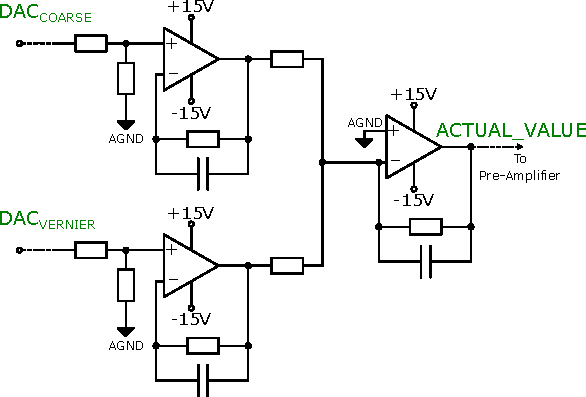
\includegraphics[width=0.8\textwidth]
    {figures/prototype/setpoint_summing_point}
    \caption[Summing Amplifier Circuit]{
        The summing amplifier circuit prepares the actual output value signal by
        scaling and combining vernier and coarse signals generated by the FPGA
        and DACs.
    }
    \label{fig:setpoint_summing_point}
\end{figure}

The pre-amplifier then generates the deviation from the desired value (setpoint)
and feeds it into the power amplifier after proper scaling.
The power amplifier then drives the source follower by generating the
$SF_{IN}$ signal as shown in \autoref{fig:power-amplifier}.
The gain of the power amplifier is dynamically selectable according to the
expected voltage range by solid state relays controlled by the \acs{MCU}.
Lower gain values will accommodate stronger input signals, providing better
signal fidelity and minimizing noise and distortion.
Higher gain values will be used for weak input signals for better amplification.


This stage injects the feedback signal of the source-follower $SF_{FEEDBACK}$
as local feedback for fine control through the use of dedicated analog switches
($S1$, $S2$ and $S3$).

The $I_{LIMIT}$ pin of the PA95 amplifier uses a resistor on the feedback
path to limit the maximum current driven from its dedicated floating supplies
to a maximum of \SI{100}{\milli\ampere} as the current supplied to the load is
drawn from the tracking power supplies rather than from the input signal source.
This means that the source follower can provide the necessary current to drive
the load while the input source only needs to provide a small signal current.

\begin{figure}[h!]
    \centering
    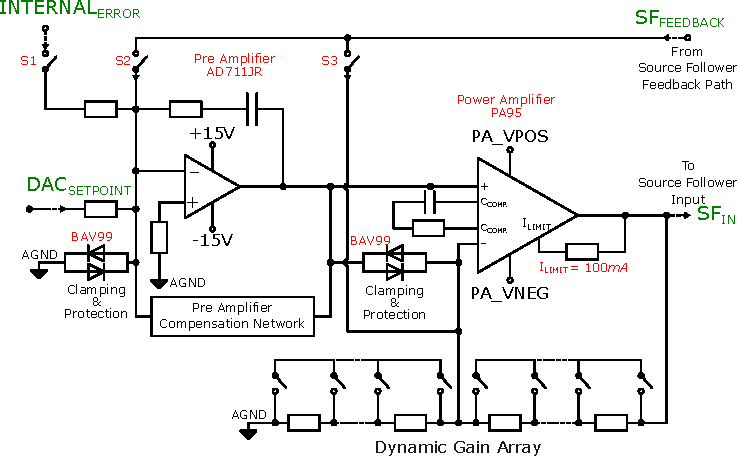
\includegraphics[width=\textwidth]
    {figures/prototype/power_amplifier}
    \caption[Power Amplifier]{
        The pre-amplifier scales the calculated error according to the
        power-amplifier requirements while the power amplifier drives the
        current-booster stage by generating the $SF_{IN}$ signal.
    }
    \label{fig:power-amplifier}
\end{figure}

\autoref{fig:current-booster-arrangement} shows the final output stage where
the required \ac{DUT} current is taken from tracking power supplies.

The output signal $SF_{OUT}$ is then fed into voltage and current measurement
blocks and the output connector while the feedback signal $SF_{FEEDBACK}$ is
optionally fed back into previous stages as a \emph{local feedback} as proposed
in \autoref{fig:system-block-diagram-hvs}.

\begin{figure}[h!]
    \centering
    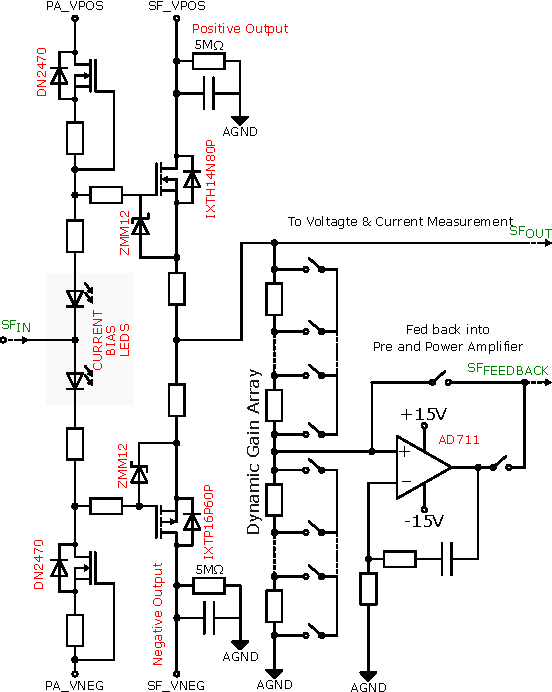
\includegraphics[width=0.8\textwidth]
    {figures/prototype/current-booster-arrangement}
    \caption[Current Booster Arrangement]{
        Simplified overview of the current booster stage implemented using
        \emph{source follower} technique.
        A pair of LEDs used for stable voltage drop and biassing current into
        the output MOSFETs gates.

    }
    \label{fig:current-booster-arrangement}
\end{figure}
